% Block diagram of Witsenhausen's counterexample, drawn top to bottom for narrow screens (phones).
% The same diagram as problem.tex. Compile to web/figures/problem-narrow.svg with:  python scripts/build_figures.py
\documentclass[tikz,border=4pt]{standalone}
\usepackage{amsmath,amssymb}
\usetikzlibrary{arrows.meta,positioning,calc}
\begin{document}
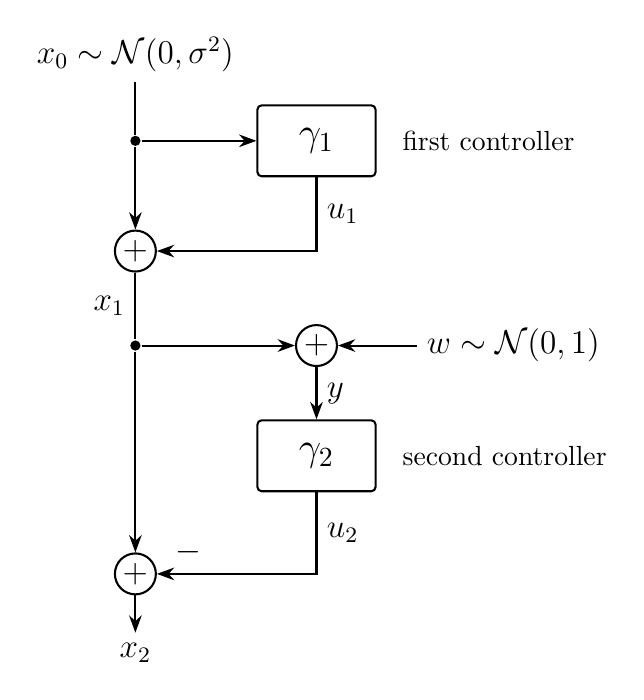
\begin{tikzpicture}[
    >={Stealth[length=2.2mm,width=1.6mm]},
    line width=0.75pt,
    font=\large,
    ctrl/.style={draw, rounded corners=1.5pt, minimum width=15mm, minimum height=9mm, align=center, font=\Large},
    sum/.style={draw, circle, inner sep=0pt, minimum size=5.2mm},
    dot/.style={circle, fill, inner sep=0pt, minimum size=1.3mm},
    ctrlname/.style={font=\normalsize},
  ]
  % plant path (left column, top to bottom)
  \node (x0)  at (0,0)     {$x_0 \sim \mathcal{N}(0,\sigma^2)$};
  \node[dot]  (b1) at (0,-1.1) {};
  \node[sum]  (s1) at (0,-2.5) {$+$};
  \node[dot]  (b2) at (0,-3.7) {};
  \node[sum]  (s3) at (0,-6.6) {$+$};
  \node (x2)  at (0,-7.6)  {$x_2$};

  % controllers and noise (right column)
  \node[ctrl] (c1) at (2.3,-1.1) {$\gamma_1$};
  \node[sum]  (s2) at (2.3,-3.7) {$+$};
  \node[ctrl] (c2) at (2.3,-5.1) {$\gamma_2$};
  \node (w) at (4.8,-3.7) {$w \sim \mathcal{N}(0,1)$};
  \node[ctrlname, right=2mm of c1] {first controller};
  \node[ctrlname, right=2mm of c2] {second controller};

  % signal flow
  \draw     (x0) -- (b1);
  \draw[->] (b1) -- (s1);
  \draw[->] (b1) -- (c1);
  \draw[->] (c1) |- node[pos=0.25, right] {$u_1$} (s1);
  \draw     (s1) -- node[left] {$x_1$} (b2);
  \draw[->] (b2) -- (s3);
  \draw[->] (b2) -- (s2);
  \draw[->] (w)  -- (s2);
  \draw[->] (s2) -- node[right] {$y$} (c2);
  \draw[->] (c2) |- node[pos=0.25, right] {$u_2$} node[pos=0.9, above] {$-$} (s3);
  \draw[->] (s3) -- (x2);
\end{tikzpicture}
\end{document}
